\documentclass[UTF8]{article}
\usepackage{ctex}
\usepackage{ulem}
\usepackage{amssymb}
\usepackage{amsmath}
\usepackage{graphicx}
\newtheorem{thm}{定义}[section]
\newtheorem{notation}[thm]{记号}
\newtheorem{lemma}[thm]{引理}

\makeatletter
\newcommand{\rmnum}[1]{\romannumeral #1}
\newcommand{\Rmnum}[1]{\expandafter\@slowromancap\romannumeral #1@}
\makeatother

\title{9 以定义扩展$\lambda{\rm C}$\\Extension of $\lambda{\rm C}$ with definitions\\[2ex]\begin{large}读书笔记\end{large}}
\author{许博}
\date{}

\begin{document}
\maketitle
	\section{$\lambda{\rm C}$扩展到系统$\lambda{\rm D_0}$}
	\noindent
	本章在$\lambda{\rm C}$的基础上扩展通常意义上定义的形式化版本,也即所谓的描述性定义(descriptive definitions)。扩展后的系统$\lambda{\rm D_0}$尚不能完全支持公理以及公理概念的表示,相应的扩展会在下一章引入$\lambda{\rm D}$时说明。
	
		为给出$\lambda{\rm D_0}$的合适的描述,首先扩展表达式的集合。$\lambda{\rm D_0}$中的表达式与$\lambda{\rm D}$中相同,因此记集合为$\mathcal{E}_{\lambda{D}}$。
		
		假设除了之前定义的变量集合$V$以外,还有常量的集合$C$。使用符号$a,a_1,a_i,a',b,...$作为常量的名字,正如我们使用$x,x_1,x_i,x',y,...$作为变量的名字一样。另外,还假设变量和常量来自不相交的集合,而$*$和$\square$是特殊符号,不属于$V$和$C$:
		
		$V\cap C=\emptyset,\ *\not=\square,\ *,\square\notin V\cup C$
		
		\begin{thm}($\mathcal{E}_{\lambda{D}}$)
			
			$\mathcal{E}_{\lambda{D}}=V|\square|*|(\mathcal{E}_{\lambda{D}}\mathcal{E}_{\lambda{D}})|(\lambda V:\mathcal{E}_{\lambda{D}}.\mathcal{E}_{\lambda{D}})|(\Pi V:\mathcal{E}_{\lambda{D}}.\mathcal{E}_{\lambda{D}})|C(\overline{\mathcal{E}_{\lambda{D}}})$
		\end{thm}
	
		其中$\overline{\mathcal{E}_{\lambda{D}}}$中的上划线表示这是一个$\mathcal{E}_{\lambda{D}}$-表达式的列表。
		
		引入“环境,environment”表示一个定义的列表。
		
		\begin{thm}($\lambda{\rm D_0}$中的描述性定义;环境)
			
			\noindent
			(1) 在$\mathcal{E}_{\lambda{D}}$中,一个(描述性)定义具有形式
			
			$\overline{x}:\overline{A}\triangleright a(\overline{x}):=M:N$
			
			\noindent
			其中所有的$x_i\in V,a\in C$,并且所有的$A_i,M,N\in\mathcal{E}_{\lambda{D}}$
			
			\noindent
			(2) 一个环境$\Delta$是一个有限(空或非空)的定义列表。
		\end{thm}
	
		使用诸如$\mathcal{D},\mathcal{D}_i,...$等符号作为元名称表示定义。一个长度为$k$的环境可以被表示为如$\Delta\equiv\mathcal{D}_1,...,\mathcal{D}_k$。
		
		关于定义,区分以下元素:
		
		\begin{thm}(定义中的元素)
			
			\noindent
			令$\mathcal{D}\equiv\overline{x}:\overline{A}\triangleright a(\overline{x}):=M:N$是一个定义。则:\\
			- $\overline{x}:\overline{A}$是$\mathcal{D}$中的上下文\\
			- $a$是$\mathcal{D}$中被定义的常量,$\overline{x}$是参数列表\\
			- $a(\overline{x})$是$\mathcal{D}$中的$definiendum$\\
			- $M:N$是$\mathcal{D}$中的语句,$M$是$definiens$或$\mathcal{D}$的主体,$N$是$\mathcal{D}$的类型。
		\end{thm}

	\section{以定义扩展推定}
	\noindent
	回顾$\lambda{\rm C}$中的推定,具有如下形式:
	
		$\Gamma\vdash M:N$
		
		但在$\lambda{\rm D_0}$中,这样的一个推定可能会依赖一些定义,因此我们在推定之前添加环境,使用元符号“;”分割环境与推定,因此包含定义的推定具有新的形式:
		
		\begin{thm}(包含定义的推定;扩展后的推定)
			
			$\Delta;\Gamma\vdash M:N$,\\
			其中$\Delta$是一个环境,$\Gamma$是一个上下文以及$M,N\in\mathcal{E}_{\lambda{D}}$。
		\end{thm}
	
		其含义为:“在环境$\Delta$和上下文$\Gamma$中,$M$具有类型$N$”。
		
		因此$M:N$由在其头部的列表$\Delta$和$\Gamma$修饰:\\
		(1) 环境$\Delta$绑定了$M:N$中出现的常量,\\
		(2) 上下文$\Gamma$绑定了$M:N$中出现的自由变量。
		
		在整个推定中,存在依赖关系,先出现的变量或常量可能会出现在之后出现的部分中,而后出现的变量或常量则不会出现在之前出现的部分中,尽管前后可能存在相同的名称,但并非表示的不同。
		
		与上下文相同,使用$\Delta,\mathcal{D}$表示在$\Delta$右边以$\mathcal{D}$进行扩展。
		
		因为暂且不考虑递归定义,因此在一个定义当中,被定义的常量只出现一次。
		
		再给出修改后的全部推到规则之前,将先引入规则($def$)和($inst$),前者导入新的定义到已存在的环境中,而后者则是定义的实例化规则。
		
	\section{用于添加定义的规则}
	\noindent
	首先,描述如何扩展一个推定中的环境$\Delta$,它已被接受并且为正确的:
	
		(\rmnum{1}) $\Delta;\Gamma\vdash K:L$
		
		在其中添加一个新的并且良构的定义,需要保证添加的定义本身是良构的,考虑如下一个新的定义:
		
		$\mathcal{D}\equiv\overline{x}:\overline{A}\triangleright a(\overline{x}):=M:N$\\
		期望将其添加至$\Delta$的尾部。
		
		因为$\Delta$中定义的常量,可能会出现在$\mathcal{D}$中,为了使$\mathcal{D}$是可接受的,需要$M:N$在上下文$\overline{x}:\overline{A}$以及环境$\Delta$中是可推导的。
		
		因此我们需要一个条件:
		
		(\rmnum{2}) $\Delta;\overline{x}:\overline{A}\vdash M:N$
		
		从而我们得到了规则(def):
		
		\begin{thm}(用于添加一个定义到一个环境中的推到规则)
			
			\noindent
			令$a$是一个未在$\Delta$中定义的新名字,且$\mathcal{D}\equiv\overline{x}:\overline{A}\triangleright a(\overline{x}):=M:N$
			
			(def) $\cfrac{\Delta;\Gamma\vdash K:L\ \ \ \Delta;\overline{x}:\overline{A}\vdash M:N}{\Delta,\mathcal{D};\Gamma\vdash K:L}$
		\end{thm}

	\section{用于实例化定义的规则}
	\noindent
	在实例化定义时,实例化一个参数可能会改变声明列表中的类型,因为定义中的上下文中后面出现的类型,可能依赖之前的声明,考虑一个具有如下形式的定义:
	
		$\mathcal{D}\equiv x_1:A_1,...,x_n:A_n\triangleright a(x_1,...,x_n):=M:N$
		
		对于每个变量$x_i$,使用表达式$U_i$进行实例化。对于$U_1$,实例化$x_1$时,需要满足条件$U_1:A_1$。而对于$U_2$,因为$A_2$可能依赖$x_1$,所以需要进行替换,因此$U_2$需要满足条件$U_2:A_2\left[x_1:=U_1\right]$。因此$U_3:A_3\left[x_1:=U_1,x_2:=U_2\right]$,需要注意的是,因为$x_1$到$x_n$都是$\mathcal{D}$中上下文的变量,因此$x_i$并不出现在$\mathcal{D}$之外,所以替换时同时替换还是顺序替换并不影响替换的结果。
		
		以此类推,对于$U_i$,需要满足条件$U_i:A_i\left[x_1:=U_1,...,x_{i-1}:=U_{i-1}\right]$。因为$x_i,...,x_n$不会出现在$A_i$中,所以对于每个表达式$U_i$所需条件的通用格式为:
		
		$U_i:A_i\left[x_1:=U_1,...,x_n:=U_n\right]$
		
		套用之前的缩写形式,使用$\left[\overline{x}:=\overline{U}\right]$作为替换$\left[x_1:=U_1,...,x_n:=U_n\right]$的缩写。因此对于每个$U_i$,应有$U_i:A_i\left[\overline{x}:=\overline{U}\right]$。再次使用上划线,以$\Delta;\Gamma\vdash\overline{U}:\overline{V}$作为列表$\Delta;\Gamma\vdash U_1:V_1,...,\Delta;\Gamma\vdash U_n:V_n$的缩写,此时规则的$\bf premisses$被缩写为$\Delta;\Gamma\vdash\overline{U}:\overline{A\left[\overline{x}:=\overline{U}\right]}$。
		
		而因为$a(\overline{x}):N$,因此$a(\overline{U}):N\left[\overline{x}:=\overline{U}\right]$,因此可以得到实例化规则(的一部分,因为不包括无参数的定义实例化):
		
		\begin{thm}(用于实例化的规则,1)
			
			\noindent
			令$a$为一个没有参数列表的常量,令$\mathcal{D}\in\Delta$,其中$\mathcal{D}\equiv\overline{x}:\overline{A}\triangleright a(\overline{x}):=M:N$,则:
			
			(inst-pos) $\cfrac{\Delta;\Gamma\vdash\overline{U}:\overline{A\left[\overline{x}:=\overline{U}\right]}}{\Delta;\Gamma\vdash a(\overline{U}):N\left[\overline{x}:=\overline{U}\right]}$
		\end{thm}
	
		其中 pos 意为 positive,正数。
		
		对于没有参数列表的定义,$\bf premisses$ 会为空,此时无法保证 $\bf conclusion$ 中$\Delta;\Gamma$的良构与否(前文中规定由$\bf premisses$保证)。故此时添加一条简单的$\bf premiss$,以保证$\Delta;\Gamma$是良构的:
		
		\begin{thm}(用于实例化的推导规则,2)
			
			\noindent
			令$a$为无参数列表的常量,令$\mathcal{D}\in\Delta$,其中$\mathcal{D}\equiv\emptyset\triangleright a():=M:N$,则:
			
			(inst-zero) $\cfrac{\Delta;\Gamma\vdash*:\square}{\Delta;\Gamma\vdash a():N}$
		\end{thm}
	
		而将规则(inst-pos)和(inst-zero)结合便得到了规则(inst)以覆盖参数列表空和非空时的情况:
		
		\begin{thm}(用于实例化的推导规则)
			
			\noindent
			令$a$为常量,令$\mathcal{D}\in\Delta$,其中$\mathcal{D}\equiv\overline{x}:\overline{A}\triangleright a(\overline{x}):=M:N$,则:
			
			(inst) $\cfrac{\Delta;\Gamma\vdash*:\square\ \ \ \Delta;\Gamma\vdash\overline{U}:\overline{A\left[\overline{x}:=\overline{U}\right]}}{\Delta;\Gamma\vdash a(\overline{U}):N\left[\overline{x}:=\overline{U}\right]}$
		\end{thm}

	\section{定义展开以及$\delta$-变换($\delta$-conversion)}
	\noindent
	关于定义有一个重要的方面还没有形式化:使用被定义的常量表示定义的实体。也即需要形式化在定义了一个常量之后,常量和实体之间需要可以互相替换。
		
		与$\beta$-规约类似,我们首先引入单步定义展开或称$\delta$-规约,需要注意的是,这个展开始终关联于定义所出现的环境$\Delta$。
		
		\begin{thm}(单步定义展开;单步$\delta$-规约,$\stackrel{\Delta}{\rightarrow}$)\\
			若$\Gamma\triangleright a(\overline{x}):=M:N$是环境$\Delta$中的一个元素,则:\\
			(1) (Basis) $a(\overline{U})\stackrel{\Delta}{\rightarrow}M\left[\overline{x}:=\overline{U}\right]$\\
			(2) (Compatibility) 若$M\stackrel{\Delta}{\rightarrow}M'$,则$ML\stackrel{\Delta}{\rightarrow}M'L,LM\stackrel{\Delta}{\rightarrow}LM',\lambda x.M\stackrel{\Delta}{\rightarrow}\lambda x.M'$以及$b(...,M,...)\stackrel{\Delta}{\rightarrow}b(...,M',...)$
		\end{thm}
	
		其中 Compatibility (2) 将是 (1) 扩展到子表达式。以及符号$\stackrel{\Delta}{\rightarrow}$简写了$\stackrel{\Delta}{\rightarrow}_\beta$。$\delta$-规约与$\beta$-规约的区别在于,每次$\delta$-规约只替换一个定义的一次出现,而$\beta$-规约则替换所有相同的绑定变量。
		
		$\stackrel{\Delta}{\rightarrow}$的逆关系被称作(单步)折叠(folding):若$M\stackrel{\Delta}{\rightarrow}M'$,则$M$是在$M'$中折叠一个确定的实例化实体的结果。
		
		与$\rightarrow_\beta$扩展到$\twoheadrightarrow_\beta,=_\beta$相似的,也定义了概念“关联$\Delta$的零或多步$\delta$-规约,$\stackrel{\Delta}{\twoheadrightarrow}$”和“关联$\Delta$的$\delta$-变换,$\stackrel{\Delta}{=}$”:
		
		\begin{thm}($\delta$-规约(零或多步),$\stackrel{\Delta}{\twoheadrightarrow}$)\\
			记$M\stackrel{\Delta}{\twoheadrightarrow}N$,若存在$n$个表达式$M_0$到$M_n$,且$M_0\equiv M$,$M_n\equiv N$以及对于所有$0\le i\lg n$有$M_i\stackrel{\Delta}{\rightarrow}M_{i+1}$。
		\end{thm}
	
		\begin{thm}($\delta$-变换,$\stackrel{\Delta}{=}$)\\
			记$M\stackrel{\Delta}{=}N$,若存$n$个表达式$M_0$到$M_n$,且$M_0\equiv M$,$M_n\equiv N$以及对于所有$0\le i\lg n$有$M_i\stackrel{\Delta}{\rightarrow}M_{i+1}$或$M_{i+1}\stackrel{\Delta}{\rightarrow}M_i$。
		\end{thm}
	
		因此,$M$和$N$是可$\delta$-变换的,当其中一个可以由另一个经过若干次的定义展开或折叠时。以及,关系$\stackrel{\Delta}{=}$具有自反性(reflexive),对称性(symmetric)和传递性(transitive)。
		
		同样,与$\beta$-规约类似,定义一个表达式的$\delta$-标准形式($\delta-normal form$),关于一个环境$\Delta$:
		
		\begin{thm}(可展开的(unfoldable),$\delta$-标准形式,$\delta$-nf)\\
			令$\Delta$是一个环境\\
			(1) 如果一个常量$a$被约束到$\Delta$中的一个描述性定义,则$a$是关于$\Delta$可展开的(unfoldable)。\\
			(2) 如果$K$中不存在关于$\Delta$可展开的常量,则$K$满足关于$\Delta$的标准形式。\\
			(3) 如果存在满足关于$\Delta$的标准形式的$L$使得$K\stackrel{\Delta}{=}L$,则$K$具有一个关于$\Delta$的标准形式。也可以说$K$是可$\delta$-标准化的,以及$L$是$K$的$\delta$-标准形式。
		\end{thm}
	
	\section{$\delta$-变换的例子}
	\noindent
	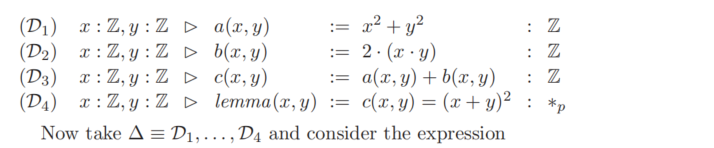
\includegraphics[width=0.93\linewidth]{"../imgs/9-1.png"}
		
		\noindent
		
\includegraphics[width=0.93\linewidth]{"../imgs/9-2.png"}
		
	\section{以$M_i\stackrel{\Delta}{\rightarrow}$扩展变换规则}
	\noindent
	在引入了$\delta$-变换之后,需要在变换规则(Conversion rule)中包含它,简单地总结出我们所期望的:
	
		如果$\Delta;\Gamma\vdash A:B$且$B\stackrel{\Delta}{=}B'$,则也有$\Delta;\Gamma\vdash A:B'$。
		
		其中$B$是良构的,因为其是已有推定的一部分,而$B'$与之前讨论中类似,不能保证其良构与否,因此我们可以得到用于$\delta$-变换的变换规则:
		
		($\delta$-conv) 如果$B\stackrel{\Delta}{=}B'$,则$\cfrac{\Delta;\Gamma\vdash A:B\ \ \ \Delta;\Gamma\vdash B':s}{\Delta;\Gamma\vdash A:B'}$。
		
		除此之外,还需要修改$\beta$-规约的定义,使其包含实例化定义参数的情况:
		
		\begin{thm}(用于$\lambda{\rm D_0}$中表达式的一步$\beta$-规约,$\rightarrow_\beta$)\\
			(1) (Basis) $(\lambda x:K.M)N\rightarrow_\beta M\left[x:=N\right]$\\
			(2) (Compatibility) 假设$M\rightarrow_\beta N$,则也有$ML\rightarrow_\beta NL,LM\rightarrow_\beta LN,\lambda x:M.K\rightarrow_\beta\lambda x:N.K,\lambda x:K.M\rightarrow_\beta\lambda x:K.N,\Pi x:M.K\rightarrow_\beta\Pi x:N.K,\Pi x:K.M\rightarrow_\beta\Pi x:K.N$以及$a(\overline{U},M,\overline{V})\rightarrow_\beta a(\overline{U},N,\overline{V})$ 
		\end{thm}
	
		$\twoheadrightarrow_\beta$和$=_\beta$的定义保持不变,因为这两者的定义依赖$\rightarrow_\beta$而非具体的表达式。
		
		现在可以给出一个组合了$\beta$-和$\delta$-变换的新的关系$\stackrel{\Delta}{=}_\beta$的定义:
		
		\begin{thm}($\beta\delta$-变换,$\stackrel{\Delta}{=}_\beta$)\\
			记$M\stackrel{\Delta}{=}_\beta N$,若存$n$个表达式$M_0$到$M_n$,且$M_0\equiv M$,$M_n\equiv N$以及对于所有$0\le i\lg n$有$M_i\rightarrow_\beta M_{i+1}$或$M_i\stackrel{\Delta}{\rightarrow}M_{i+1}$或$M_{i+1}\rightarrow_\beta M_i$或$M_{i+1}\stackrel{\Delta}{\rightarrow}M_i$。
		\end{thm}
	
		此时便可以给出适用于$\lambda{\rm D_0}$的通用变换规则:
		
		\begin{thm}(用于$\beta$-$\delta$-变换的推导规则)
			
			($\beta\delta$-conv) 如果$B\stackrel{\Delta}{=}_\beta B'$,则$\cfrac{\Delta;\Gamma\vdash A:B\ \ \ \Delta;\Gamma\vdash B':s}{\Delta;\Gamma\vdash A:B'}$
		\end{thm}
	
	\section{$\lambda{\rm D_0}$中的推导规则}
	\noindent
	其中$(s_1,s_2)$的可以为$(*,*),(\square,*),(\square,\square)$或$(*,\square)$:
	
		\noindent
		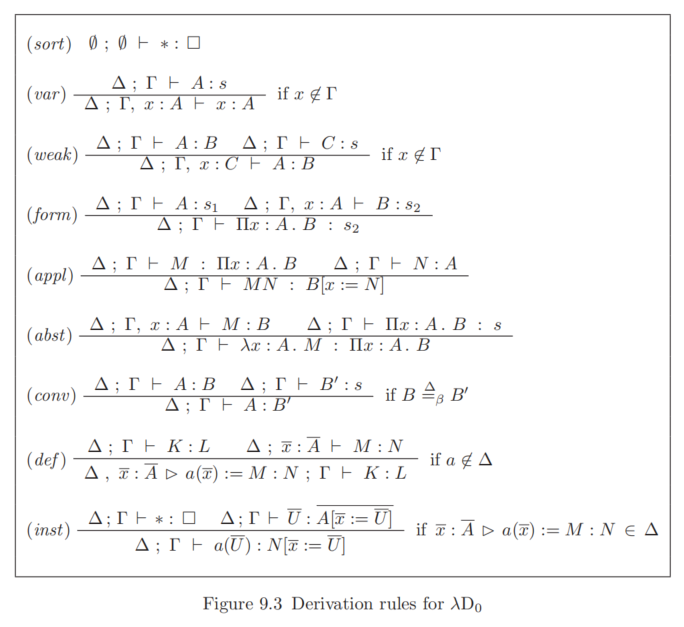
\includegraphics[width=0.93\linewidth]{"../imgs/9-3.png"}
		
		其中变化之处主要在于$\Delta$的添加,定义的引入和实例化以及($conv$)规则的修改。
		
	\section{仔细研究$\lambda{\rm D_0}$的推导规则}
	\noindent
	观察($weak$)-规则和($def$)-规则,前者弱化了一个推定的上下文,在上下文的结尾添加新的声明,而后者弱化了一个推定的环境,在环境的结尾添加新的定义,两者都可以被认为是弱化规则,一个用于上下文,另一个用于环境。
	
		再观察规则($var$)和规则($inst$),前者告诉了我们一个变量的类型是什么,变量作为上下文中最后一个声明的主体,并且它的类型是关于环境和上下文良构的;后者告诉了我们一个实例化的常量的类型是什么,类型也是关于环境和上下文良构的。因此这两个规则确定了$\lambda{\rm D_0}$中基本表达式的类型,从基本表达式开始,由其它规则构建出更加复杂的表达式。
		
		再次观察($var$)-规则,其表述在上下文中最后一个声明自身是关于一个合法的环境和上下文可推导的,而在定义相关的概念中,并没有类似的规则,也即“最后一个定义是关于一个合法的环境和上下文可推导的”,因为定义并不是一个语句,不满足出现在$\vdash$之后的格式要求。但可以从定义中提取出两个可接受的语句,也即$a(\overline{x}):N$和$M:N$,两者都是合法的语句,其中后者可以由($def$)-规则的第二个$\bf premiss$直接得到,后一个语句可推导则通过引入($par$)-规则:
		
		($par$) 如果$\mathcal{D}\equiv\overline{x}:\overline{A}\triangleright a(\overline{x}):=M:N$且$a\notin\Delta$,则$\cfrac{\Delta;\overline{x}:\overline{A}\vdash M:N}{\Delta,\mathcal{D};\overline{x}:\overline{A}\vdash a(\overline{x}):N}$
		
		需要注意的是这条规则不属于基础规则,同时在我们的理论研究中不需要考虑它。
\end{document}
